\documentclass[12pt]{article}
\usepackage{url}
\usepackage{latexsym}
\usepackage{multirow}
\usepackage{graphicx}
\graphicspath{}
\usepackage{subfig}
\usepackage{booktabs}
\usepackage{natbib}
\usepackage{float}
\usepackage{listings}
\lstset{ 
 breaklines = true,
 extendedchars=false, 
 xleftmargin=2em,xrightmargin=2em, aboveskip=1em, 
 tabsize=4,
 showspaces=false 
 }


\title{Exploring on how could Developers Excavate Useful Information in Steam Reviews}

\author{Jiyan CHEN \\ \\
Data and Social Media Analysis: Final Report \\ {\tt chin\_kigen@toki.waseda.jp}}


\date{2022/02/01}

\begin{document}
\maketitle
\begin{abstract}
Steam reviews is one factor of making Steam a valuable resource for developers. However, Steam reviews has some short comes that make the data hard to be use directly since the noise. This article take the game \textsl{No Man's Sky} as an example by using technique of visualization, topic modeling, to explore how can game developers dig useful information from reviews with noise.
\end{abstract}


\section{Introduction}
\label{intro}

Steam is a massive video game distribution platform. According the official statistic data, steam has over 120 millions monthly active users since 2020. The game developers could easily get tons of reviews of their games through this platform. 

However, Steam reviews has various problems such as the displaying only aggregation of all the reviews about a game which makes crucial reviews being dismissed since it being put on in 2013, that makes the reviews of game hard to be make use of by the developers.

In this article choose the game \textsl{No Man's Sky} published by Hello Games as a target. \textsl{No Man's Sky} has been chosen as the most disappointing game of 2016 by most video game media and received a 'mostly negative' on Steam which means it only has less than 30 percent positive reviews among all the reviews. Nevertheless, after 5 years of updating, its reviews ticked over into ‘mostly positive’ territory in 2021.

By analyzing the reviews of \textsl{No Man's Sky} collected through the official API provided by Valve, this article would like to discuss if there are some methods for the developers to excavate valuable information among millions of reviews. 

In the following section, the research background would be introduced. Then the method and analyzing result of the data would be demonstrated. Finally, this article would like to discuss about the conclusion and the points which needs a further research to be taken.

\section{Background}
\label{label:background}
Ian Boudreau, an editor of \textsl{PCGamesN}, pointed out three main problem with current Steam review system. Firstly, Steam reviews are shown in the format of aggregation which makes the user not able to see the detail opinions, in which way crucial information and context being covered. Secondly, game may have a low rating for some misinformed or wildly inaccurate reasons that is not related to the game content itself. Thirdly, the negative reviews may have a further influence on the game rating even if the issue it mentioned has been solved. However, Boudreau still praised Steam review as a main approach for developers to collect player's feedback. \citep{boudreau_2021} Therefore, this article would explore on how to excavate useful information among the reviews with a lot of noise. 

\section{Data and Method}
\label{Data-method}
The data set is download from kaggle which is collected through the official API offered by Valve. The data set concludes the reviews until October 2020 since \textsl{No Man's Sky} is released.
Table \ref{Tab:API} shows the basic information of the data set.

\begin{table}[H]
    \centering
    \caption{Steam API Instruction}
    \begin{tabular}{lp{0.6\columnwidth}lp{0.8\columnwidth}}
    \toprule
    \textbf{Name}                                                                                          & \textbf{Description}                                                            \\ \midrule
    \textbf{review}                                                                                        & text of written review                                                 \\[+3pt]
    \textbf{timestamp\_created}                                                                            & date the review was created (unix timestamp)                           \\[+3pt]
    \textbf{timestamp\_updated}                                                                            & date the review was last updated (unix timestamp)                      \\[+3pt]
    \textbf{voted\_up}                                                                                     & \textbf{True} means it was a positive recommendation                            \\[+3pt]
    \textbf{votes\_valuable}                                                                               & the number of users that found this review helpful                     \\[+3pt]
    \textbf{votes\_funny}                                                                                  & the number of users that found this review funny                       \\[+3pt]
    \textbf{weighted\_vote\_score}                                                                         & helpfulness score                                                      \\[+3pt]
    \textbf{comment\_count}                                                                                & number of comments posted on this review                               \\[+3pt]
    \textbf{received\_for\_free}                                                                           & \textbf{True} if the user checked a box saying they got the app for free        \\[+3pt]
    \textbf{written\_during\_early\_access}                                                                & \textbf{True} if the user posted this review while the game was in Early Access \\[+3pt]
    \textbf{author.num\_games\_owned}                                                                      & number of games owned by the user                                      \\[+3pt]
    \textbf{author.num\_reviews}                                                                           & number of reviews written by the user                                  \\[+3pt]
    \textbf{author.playtime\_forever}                                                                      & lifetime playtime tracked in this app                                  \\[+3pt]
    \textbf{author.playtime\_last\_two\_weeks}                                                             & playtime tracked in the past two weeks for this app                    \\[+3pt]
    \textbf{author.playtime\_at\_review}                                                                   & playtime when the review was written                                   \\[+3pt]
    \textbf{author.last\_played}                                                                           & time for when the user last played (unix timestamp)                    \\
    \bottomrule
    \end{tabular}
    \label{Tab:API}
\end{table}

This article uses plots such as bar plot, histogram, and heat map to display and make analysis on the numerical data including the player count, playtime and timestamp. Also, several word cloud are created to demonstrate the most common words being used. In order to find possible topics hidden in the reviews, LDA topic modeling has been conducted, and the result of topic modeling is visualized through wordcloud and pyLDAvis. To make LDA topic modeling on the text, the reviews would be prepossessed through methods including text cleaning, tokenization, stopwords removing and lemmatization. This article use coherence score used to judge the performance of the model, and find the most fitted model through iterate the parameter for topic numbers.

\section{Results}

\begin{figure}[H]
\centering
\subfloat[All users]{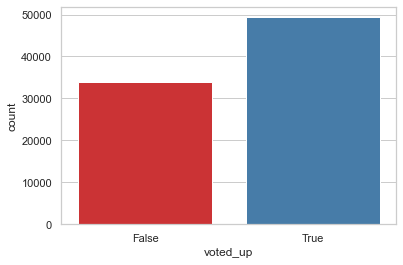
\includegraphics[width=0.48\linewidth]{images/all user.png}}
\hfill
\subfloat[Users have updated reviews]{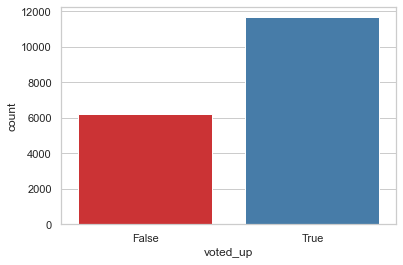
\includegraphics[width=0.48\linewidth]{images/user updated.png}}
\caption{Bar-plot Users' Reviews}
\label{fig:bar}
\end{figure}

\begin{figure}[H]
\centering
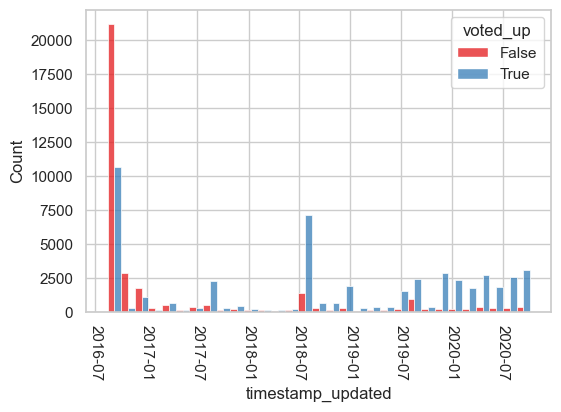
\includegraphics[scale=0.7]{images/timestamp.png}
\caption{Votes by time updated}
\label{fig:timestamp}
\end{figure}

\begin{figure}[H]
\centering
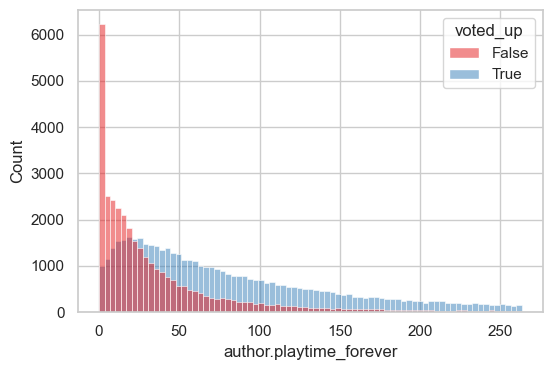
\includegraphics[scale=0.7]{images/forever.png}
\caption{User's total playtime}
\label{fig:forever}
\end{figure}

\begin{figure}[H]
\centering
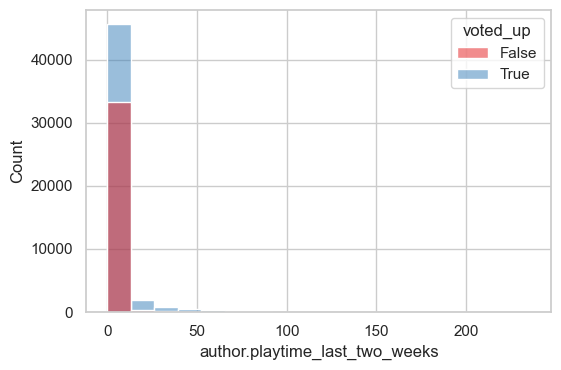
\includegraphics[scale=0.7]{images/last two weeks.png}
\caption{User's playtime last two weeks}
\label{fig:last two weeks}
\end{figure}

\begin{figure}[H]
\centering
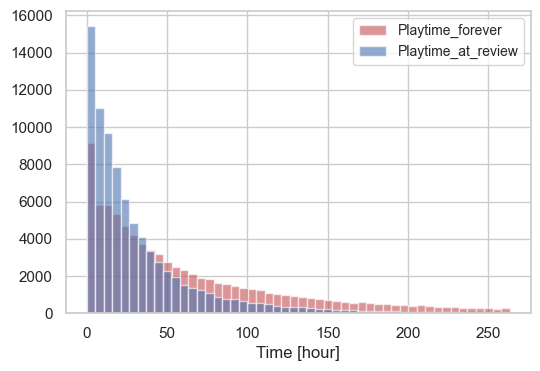
\includegraphics[scale=0.7]{images/forever v at_review.png}
\caption{User's total playtime compared to playtime at review}
\label{fig:forever v at_review}
\end{figure}

\begin{figure}[H]
\flushleft
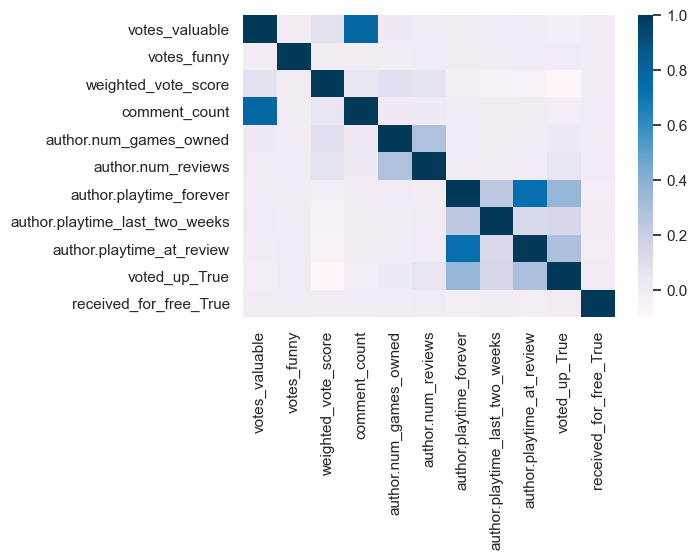
\includegraphics[scale=0.70]{images/heatmap.png}
\caption{Heat map}
\label{fig:heatmap}
\end{figure}

\begin{figure}[H]
  \centering
  \subfloat[All users]{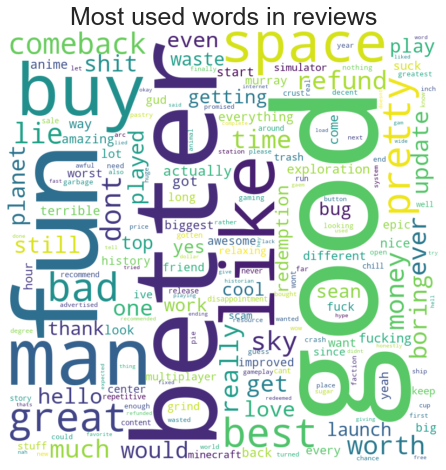
\includegraphics[scale=0.4]{images/wordcloud all.png}\label{fig:1}}

  \subfloat[Users Vote for Positive]{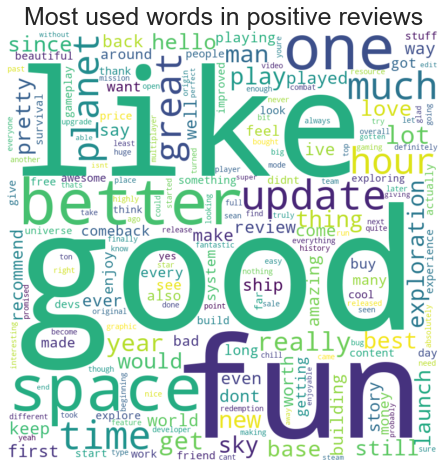
\includegraphics[scale=0.4]{images/wordcloud positive.png}\label{fig:2}}\hspace{1em}
  \subfloat[Users Vote for Negative]{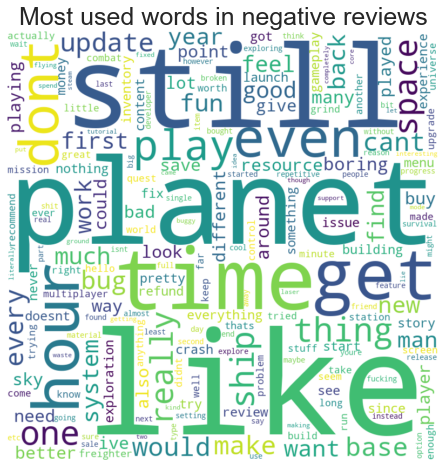
\includegraphics[scale=0.4]{images/wordcloud negative.png}\label{fig:3}}
  \caption{Wordcloud of Users' Reviews}
\end{figure}

\begin{figure}[H]
\centering
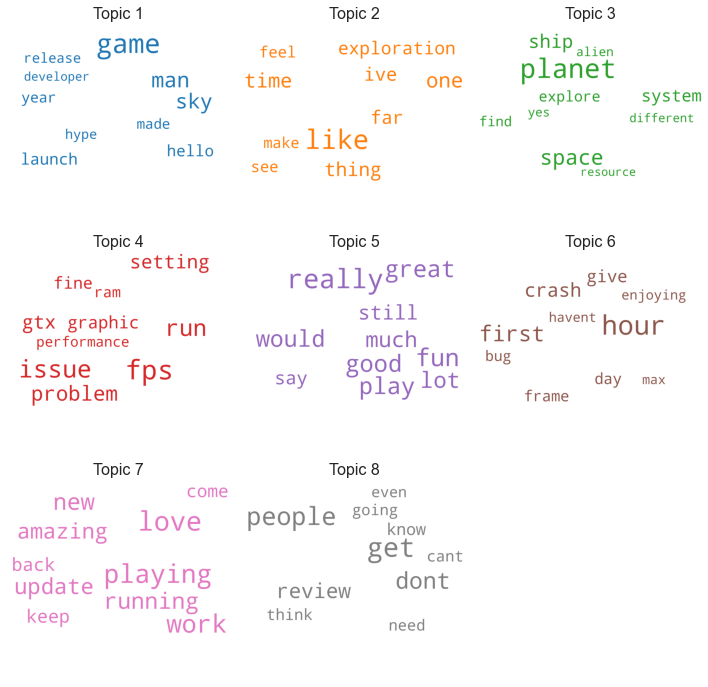
\includegraphics[scale=0.6]{images/topic_positive.png}
\caption{Wordcloud for topic modeling on positive reviews}
\label{fig:wordcloudp}
\end{figure}

\begin{figure}[H]
\centering
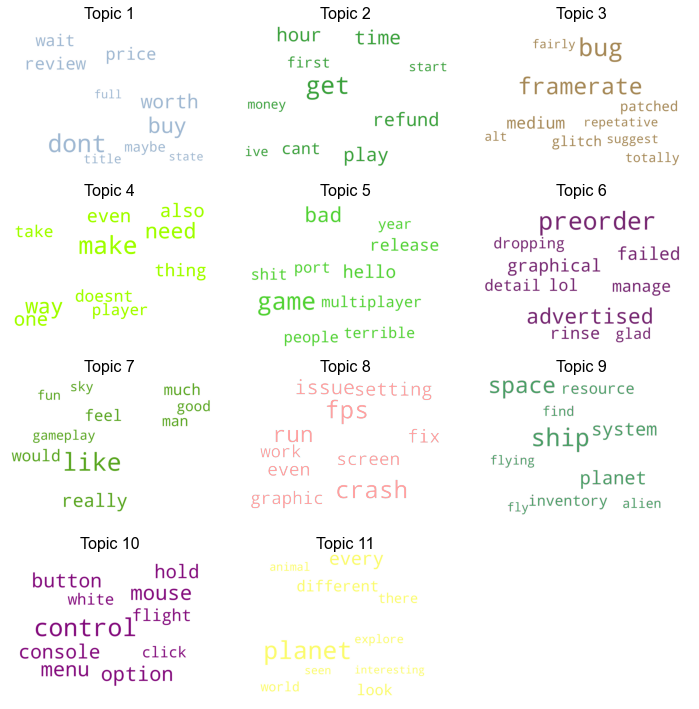
\includegraphics[scale=0.6]{images/topic_negative.png}
\caption{Wordcloud for topic modeling on negative reviews}
\label{fig:wordcloudn}
\end{figure}

\newpage
\section{Conclusion and Discussion}
\label{Conlusion}
From figure \ref{fig:bar}, compare to all the users, users that have updated their reviews after several hours of gameplaying are more likely to give a positive feedback.

Figure \ref{fig:timestamp} shows the histogram of review counts by the last time user updated their reviews. According to the plot, the negative reviews concentrate in the first half year that the game was released. The following updates' positive feedback rate is over 90 percent. However, the aggregation positive feedback rate of all the reviews takes two years to tick over 'mixed'(over 40\%),and just reach 'mostly positive'(over 70\%) in 2021. This indicates a big problem of Steam review system point out by Ian Boudreau that even the factors mentioned by the negative reviews has been improved, the aggregation positive feedback rate still could keep at a low level for a long time.

figure 3,4 is the histogram of users' playtime total and last two weeks separately, as the chart shows, users who give positive feedback have longer average playtime than a user who gives negative feedback. The heat map in figure 6 shows the same result as well. Notice that most player who gives negative feedback has a very short total playtime which could indicate that their reviews may not be very helpful for the improvement of the game content.


Through figure 5 it can be inferred that many players give their reviews when they do not actually deeply experienced most even half of the game content. If look at the reviews, there would be a lot of reviews that just simply give a simple word such as good, pretty, bad, and terrible instead of state specific information about the point which makes a good game or a bad game. In 2019's Game Developers Conference(GDC 2019), which is one of the biggest conferences for game developers, the founder of Hello Game Sean Murray made a speech about the experience of developing No Man's Sky. According to the speech, Sean Murray says that 80 percent of player who has sent an email that gives negative feedback does not really played the game. Therefore, a reason for many players to give their reviews when they do not fully experienced the game may be driven by the herd mentality. 

Figure 7 shows three word cloud generated from the text after processed by all the reviews, positive, and negative reviews separately. The most common words in positive reviews are some normal commendatory term such as 'good', 'fun', 'great'. But notice that 'update' is a relatively common word in positive reviews, which indicates that the updates could meet a considerable part of players' requirement. Also, 'planet' is a very useful word in positive reviews, which is connected with the game content. However, through only planet developers can hardly get the detail point of the advantage about the game content, so it is necessary to combine the result with the result of topic modeling. Same regarding to the negative reviews, 'planet' is one of the most common word being used, it need the result of topic modeling for exploring more details. 

Figure \ref{fig:wordcloudp} and \ref{fig:wordcloudn} are the results of topic modeling on positive, negative reviews with the highest coherence score. Apparently, topic 4 in Figure \ref{fig:wordcloudp} is about game optimization especially on graphic, since it includes words like 'fps'(frame per second),'gtx'(a Nvidia Graphics card series). This topic is corresponding with topic 8 in Figure \ref{fig:wordcloudn}. Also, topic 6 in in Figure \ref{fig:wordcloudp} is likely to be about bugs found in games, and topic 3 in Figure \ref{fig:wordcloudn} mentioned this problem as well. In Figure \ref{fig:wordcloudn} for the result of negative reviews, a lot of topics that has little thing to do with the game content can be found such as topic 2 which seems just talking about refunding, topic 6 is about the game's marketing and regretting about preorder. However, the result shows some point that gives the developer idea how to improve game. Topic 5 mentioned about the multiplayer game which was cut off by the release of the game. Also, topic 10 mentioned about the problem on controlling and user interface in the game. What is more, topic 9 mentioned about some defect among the game's system for example inventory and space ship. In addition topic 11 is about the requirement of new planet content.

Overall, the Steam review does contain a lot of noise information which prevent the game developer to get useful information for improve the game. Nevertheless, topic modeling developer could become a method for the developers to get some direction from millions of reviews. Take No man's sky as an example, developer could possibly improve their game on field such as game optimization, bug fixing, multiplayer mode, controlling and user interface, system and new content. For Steam platform, if it can be take into consider that add some more class to give user more option to vote for specific field, which could reduce the influence from factors other than the game content. Also, the platform could keep player's review, and ask if the player wants to update it after the player has played the game for hours.




\section{Future Work}
\label{future}
This article conducted an exploration on analysing reviews through LDA topic modeling, and the result could give developers some guidance on how to improve the game. However, use wordcloud to display the result could only gives common words in each topics. In this case, a better way to demonstrate the result of modeling is worth researching. Also, it needs to be verified if modeling on text separated by sentimental analysis could improve performance of the model. 
\section{List of tools and methods used}
The tools and code used in this article is listed below.
\subsection{Tools and software}
\begin{itemize}
\item Python3
\begin{itemize}
\item NLTK
\item re
\item gensim
\item pandas
\item numpy
\item wordcloud
\item spacy
\item demoji
\item string
\item collections
\item pyLDAvis
\item seaborn
\item matplotlib
\end{itemize}
\end{itemize}
\subsection{Code}
\scriptsize
\begin{lstlisting}[language = Python]
import re
import numpy as np
import pandas as pd
from pprint import pprint
import datetime

# Gensim and LDA
import gensim
import gensim.corpora as corpora
from gensim.utils import simple_preprocess
from gensim.models import CoherenceModel
from gensim.parsing.preprocessing import STOPWORDS
import pyLDAvis
import pyLDAvis.gensim_models as gensimvis
pyLDAvis.enable_notebook()

# NLP
import demoji
import string
import nltk
from wordcloud import WordCloud 
from nltk.stem import WordNetLemmatizer, SnowballStemmer
from nltk.stem.porter import *
import spacy
import collections
from collections import Counter

# plot
import matplotlib.colors as mcolors
import matplotlib.pyplot as plt
import seaborn as sns
%matplotlib inline

df = pd.read_csv('275850_NoMansSky.csv', index_col=0, usecols = [0,3,4,5,6,7,8,9,10,12,13,15,16,17,18,19,20])
df = df.rename(columns={'votes_up':'votes_valuable'})
df.head()

df.dropna(axis=0, how='any', inplace=True)

df.info()

df.isnull().sum()

df['timestamp_created'] = df['timestamp_created'].apply(lambda x: datetime.datetime.fromtimestamp(x))
df['timestamp_updated'] = df['timestamp_updated'].apply(lambda x: datetime.datetime.fromtimestamp(x))
df['author.last_played'] = df['author.last_played'].apply(lambda x: datetime.datetime.fromtimestamp(x))
df.head()

df['author.playtime_forever'] = df['author.playtime_forever'].apply(lambda x: x/60)
df['author.playtime_last_two_weeks'] = df['author.playtime_last_two_weeks'].apply(lambda x: x/60)
df['author.playtime_at_review'] = df['author.playtime_at_review'].apply(lambda x: x/60)

sns.boxplot(data = df.iloc[:,[12,13]])

def remove_outlier(df_in, col_name):
    q1 = df_in[col_name].quantile(0.25)
    q3 = df_in[col_name].quantile(0.75)
    iqr = q3-q1 #Interquartile range
    fence_low  = q1-1.5*iqr
    fence_high = q3+1.5*iqr
    df_out = df_in.loc[(df_in[col_name] > fence_low) & (df_in[col_name] < fence_high)]
    return df_out
    
df_flitered = pd.DataFrame()
df_flitered = remove_outlier(df,'author.playtime_forever')

sns.countplot(x="voted_up", data=df_flitered)
plt.ticklabel_format(style='plain', axis='y')
plt.show()

sns.countplot(x="voted_up", data=df_flitered[df_flitered['timestamp_created']!=df_flitered['timestamp_updated']])
plt.ticklabel_format(style='plain', axis='y')
plt.show()

sns.set()
sns.set_style('whitegrid')
sns.set_palette('Set1')
plt.figure(dpi=100)
plt.xticks(rotation = 270)
sns.histplot(data=df_flitered, x='timestamp_updated',hue='voted_up',multiple='dodge')

sns.set()
sns.set_style('whitegrid')
sns.set_palette('Set1')
plt.figure(dpi=100)
sns.histplot(data=df_flitered, x='author.playtime_forever', hue='voted_up')

plt.figure(dpi=100)
sns.histplot(data=df_flitered, x='author.playtime_last_two_weeks', hue='voted_up')

fig = plt.figure(dpi=100)
ax = fig.add_subplot(1, 1, 1)
ax.hist(df_flitered['author.playtime_forever'], bins=50, alpha=0.6,color='r',label='Playtime_forever')
ax.hist(df_flitered['author.playtime_at_review'], bins=50, alpha=0.6, color='b',label='Playtime_at_review')
ax.set_xlabel('Time [hour]')
ax.legend(loc="upper right", fontsize=10)
plt.show()

dfR = pd.get_dummies(df_flitered,columns=['voted_up','received_for_free','written_during_early_access'],drop_first=True)
dfR

plt.figure(dpi=100)
sns.heatmap(dfR.corr(),cmap="PuBu")

from nltk.corpus import stopwords
stop_words = stopwords.words('english')

stop_words.extend(['game'])

def preprocess(text):
    
    # change all the capital words to lower
    text = text.apply(lambda x: ' '.join([w.lower() for w in x.split()]))
    # replace all the emoji by demoji
    text = text.apply(lambda x: demoji.replace(x, ''))
    # remove punctuations
    text = text.apply(lambda x: ''.join([i for i in x if i not in string.punctuation]))
    # remove number and special characters
    text = text.apply(lambda x: ' '.join(re.sub("[^a-zA-Z]+", " ",x).split()))
    # remove stopwords
    text = text.apply(lambda x: ' '.join([w for w in x.split() if w not in stop_words]))
    # lemmatization
    text = text.apply(lambda x: ' '.join([WordNetLemmatizer().lemmatize(w) for w in x.split()]))
    # remove words less than 3 characters
    text = text.apply(lambda x: ' '.join([w.strip() for w in x.split() if len(w.strip()) >= 3]))
    
    return text

df_flitered["review_preprocessed"] = preprocess(df_flitered['review'])

df_flitered.head()

def WordCloud_generator(data, title=None):
    
    most_freq = Counter(data).most_common(1000) 
    text = ' '.join([x[0] for x in most_freq])
    
    wordcloud = WordCloud(stopwords= stop_words, width = 800, height = 800,
                          background_color ='white',
                          min_font_size = 10,
                          collocations=False
                         ).generate(text)
                  
    plt.figure(figsize = (6, 6), facecolor = None) 
    plt.imshow(wordcloud, interpolation='bilinear') 
    plt.axis("off") 
    plt.tight_layout(pad = 0) 
    plt.title(title,fontsize=25)
    plt.show() 
    
WordCloud_generator(df_flitered["review_preprocessed"], title="Most used words in reviews")

WordCloud_generator(df_flitered[df_flitered["voted_up"] == True]["review_preprocessed"], title="Most used words in positive reviews")

WordCloud_generator(df_flitered[df_flitered["voted_up"] == False]["review_preprocessed"], title="Most used words in negative reviews")

Positive_doc = df_flitered[df_flitered['voted_up'] == True]['review_preprocessed'].apply(lambda x: x.split()).tolist()
id2word_P = gensim.corpora.Dictionary(Positive_doc)
id2word_P.filter_extremes(no_below=15, no_above=0.5, keep_n=100000) # Filt extreme words
Positive_doc[:1]

corpus_positive = [id2word_P.doc2bow(text) for text in Positive_doc]

def compute_coherence_values(id2word, corpus, texts, limit, start, step):
    
    coherence_values = []
    model_list = []
    for num_topics in range(start, limit, step):
        model =  gensim.models.ldamodel.LdaModel(random_state=2022, 
                                                 corpus=corpus, 
                                                 num_topics=num_topics, 
                                                 id2word=id2word,
                                                 update_every=1,
                                                 chunksize=300,
                                                 passes=10,
                                                 alpha='auto',
                                                 per_word_topics=True
                                                )
        model_list.append(model)
        coherencemodel = CoherenceModel(model=model, texts=texts, dictionary=id2word, coherence='c_v')
        coherence_values.append(coherencemodel.get_coherence())

    return model_list, coherence_values


model_list, coherence_values_positive = compute_coherence_values(id2word=id2word_P, corpus=corpus_positive, texts=Positive_doc, start=2, limit=17, step=3)

limit=17; start=2; step=3;
x = range(start, limit, step)
plt.plot(x, coherence_values_positive)
plt.xlabel("Num Topics")
plt.ylabel("Coherence score")
plt.legend(("coherence_values"), loc='best')
plt.show()

for m, cv in zip(x, coherence_values_positive):
    print("Num Topics =", m, " has Coherence Value of", round(cv, 4))
    
optimal_model_positive = model_list[2]
model_topics = optimal_model_positive.show_topics(formatted=False)
pprint(optimal_model_positive.print_topics(num_words=10))

import matplotlib.colors as mcolors

cols = [color for name, color in mcolors.TABLEAU_COLORS.items()]  # more colors: 'mcolors.XKCD_COLORS'

cloud = WordCloud(stopwords=stop_words,
                  background_color='white',
                  width=2500,
                  height=1800,
                  max_words=10,
                  colormap='tab10',
                  color_func=lambda *args, **kwargs: cols[i],
                  prefer_horizontal=1.0)

topics = optimal_model_positive.show_topics(formatted=False)

fig, axes = plt.subplots(3, 3, figsize=(10,10), sharex=True, sharey=True)

for i, ax in enumerate(axes.flatten()):
    fig.add_subplot(ax)
    if i < len(topics):
        topic_words = dict(topics[i][1])
        cloud.generate_from_frequencies(topic_words, max_font_size=300)
        plt.gca().imshow(cloud)
        plt.gca().set_title('Topic ' + str(i+1), fontdict=dict(size=16))
        plt.gca().axis('off')

plt.subplots_adjust(wspace=0, hspace=0)
plt.axis('off')
plt.margins(x=0, y=0)
plt.tight_layout()
plt.show()

vis_P = pyLDAvis.gensim_models.prepare(optimal_model_positive, corpus_positive, id2word_P)
vis_P

Negative_doc = df_flitered[df_flitered['voted_up'] == False]['review_preprocessed'].apply(lambda x: x.split()).tolist()
id2word_N = gensim.corpora.Dictionary(Negative_doc)
id2word_N.filter_extremes(no_below=15, no_above=0.5, keep_n=100000) # Filt extreme words
Negative_doc[:1]

corpus_negative = [id2word_N.doc2bow(text) for text in Negative_doc]

def compute_coherence_values(id2word, corpus, texts, limit, start, step):
    
    coherence_values = []
    model_list = []
    for num_topics in range(start, limit, step):
        model =  gensim.models.ldamodel.LdaModel(random_state=2022, 
                                                 corpus=corpus, 
                                                 num_topics=num_topics, 
                                                 id2word=id2word,
                                                 update_every=1,
                                                 chunksize=300,
                                                 passes=10,
                                                 alpha='auto',
                                                 per_word_topics=True
                                                )
        model_list.append(model)
        coherencemodel = CoherenceModel(model=model, texts=texts, dictionary=id2word, coherence='c_v')
        coherence_values.append(coherencemodel.get_coherence())

    return model_list, coherence_values


model_list_negative, coherence_values_negative = compute_coherence_values(id2word=id2word_N, corpus=corpus_negative, texts=Negative_doc, start=2, limit=17, step=3)

limit=17; start=2; step=3;
x = range(start, limit, step)
plt.plot(x, coherence_values_negative)
plt.xlabel("Num Topics")
plt.ylabel("Coherence score")
plt.legend(("coherence_values"), loc='best')
plt.show()

for m, cv in zip(x, coherence_values_negative):
    print("Num Topics =", m, " has Coherence Value of", round(cv, 4))
    
optimal_model_negative = model_list_negative[3]
model_topics = optimal_model_negative.show_topics(formatted=False)
pprint(optimal_model_negative.print_topics(num_words=10))

import matplotlib.colors as mcolors

cols = [color for name, color in mcolors.XKCD_COLORS.items()]

cloud = WordCloud(stopwords=stop_words,
                  background_color='white',
                  width=2500,
                  height=1800,
                  max_words=10,
                  colormap='tab10',
                  color_func=lambda *args, **kwargs: cols[i],
                  prefer_horizontal=1.0)

topics = optimal_model_negative.show_topics(num_topics=11,formatted=False)

fig, axes = plt.subplots(4, 3, figsize=(10,10), sharex=True, sharey=True)

for i, ax in enumerate(axes.flatten()):
    fig.add_subplot(ax)
    if i < len(topics):
        topic_words = dict(topics[i][1])
        cloud.generate_from_frequencies(topic_words, max_font_size=300)
        plt.gca().imshow(cloud)
        plt.gca().set_title('Topic ' + str(i+1), fontdict=dict(size=16))
        plt.gca().axis('off')

plt.subplots_adjust(wspace=0, hspace=0)
plt.axis('off')
plt.margins(x=0, y=0)
plt.tight_layout()
plt.show()

vis_N = pyLDAvis.gensim_models.prepare(optimal_model_negative, corpus_negative, id2word_N)
vis_N
\end{lstlisting}

\bibliographystyle{plain}%This is where the referencing style name goes
\bibliography{DSMAfinal}%This is where the name of your .bib file goes
\nocite{*}
%The references appear automatically

\end{document}
